\documentclass{article}

\usepackage{amssymb}
\usepackage{amsmath}
\usepackage{tikz} 


\begin{document}
    $\mathfrak{S}_n$

    \begin{displaymath}
        \underbrace{x^2+1}_{\text{no real root}}
    \end{displaymath}


    \begin{equation}
        \sum_{\substack{i \geq a \\ j \in A}} ij
    \end{equation}


    \begin{equation}
        \boxed{\oint _{\gamma} f(\zeta) \, d\zeta}
    \end{equation}

    \begin{equation}
        \lceil \frac{1}{2} \rceil = \left\lceil \frac{1}{2} \right\rceil
    \end{equation}
    

    \begin{align}
        x &= a + b + c \\
          &\leq \alpha + \beta + \gamma
    \end{align}

    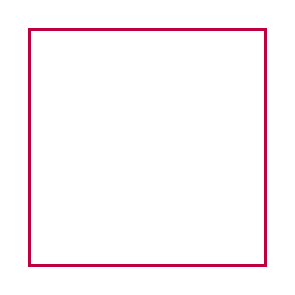
\begin{tikzpicture}
        \draw[purple, very thick] (0,0) rectangle (3,3);
    \end{tikzpicture}

    \begin{abstract}
        \noindent
        Let $\varphi$ be the golden ratio and put 

        \[\alpha = \sum_{n=1}^\infty 2^{-\lfloor n\varphi \rfloor}\]
        then 
        \[
            \alpha = \cfrac{1}{1+\cfrac{1}{2^1+\cfrac{1}{2^1+\cfrac{1}{2^2+\cfrac{1}{2^3+\cfrac{1}{2^5+\cfrac{1}{2^8+\cfrac{1}{2^{13}+\dots}}}}}}}}
        \]
        
        \noindent wherein the exponenets follow the \emph{Fibonacci sequence}!
    \end{abstract}

\end{document}